 % - IPC Functionality
 %  - Minimum required per subnet
 %    - Withdrawal/Deposits Interfaces
 %    - Other Operations? (Propagate?)
 %  - Enhancements
 %    - Checkpointing interfaces
 %    - Propagate
 %    - Reporting/Slashing interfaces
 %    - Atomic execution/swap, IBC-like bridges
 %  - Future stuff (google docs?)
 %    - Withdrawal at ancestor (skip parent(s)) (with timeout) etc.
\section{IPC functionality}
\label{sec:functionality}

IPC exposes the following functionalities:
\begin{itemize}
    \item Creating child subnets.
    \item Removing child subnets.
    \item Depositing coins from an account in a subnet to an account in its child.
    \item Withdrawing coins from an account in a subnet to an account in its parent.
    \item Checkpointing a subnet's replicated state in the replicated state of its parent.
    \item Propagating cross-net transactions.
    \item Slashing misbehaving child replicas.
\end{itemize}
In the following, we describe each functionality in detail.

\subsection{Creating a child subnet}
\label{sec:create}

Any user of a subnet $P$ can create a new subnet $P/C$ by submitting a transaction $P.\gw.CreateChild(P/C, params)$.
This results in the creation of a new subnet actor $\sa_C$ in $P$ governing the subnet $P/C$.
The \emph{params} value describes all the subnet-specific parameters required to initialize the state of $P.\sa_C$,
such as the initial membership data, the consensus protocol to use, required collateral to use, etc.

The subnet is considered created as soon as the \sa is created.
From the parent's point of view, the subnet need not yet necessarily be operational at that moment,
as the parent subnet always has a passive role when it comes to interacting with it.

\subsection{Deposits}
\label{sec:deposit}

% \del{
% \arp{Consider need to pause/remedy subnet after deposit (e.g. collateral not enough with new supply). IPC agent should check in that case}\guy{Does this comment belong here or somewhere else?}\\
% }

A deposit is a transfer of funds (of some amount \fil) from an account \src in the parent subnet $P$ to an account \dest in the child subnet $P/C$ (i.e., \dest has the form $P/C.someAccount$).
We assume that the owner of \src is either running their own IPC Agent to perform the necessary operations described below, or uses another trusted IPC agent to act on their behalf.
The deposit is performed as follows:
\begin{enumerate}
    \item The owner of \src submits a transaction
    $\tx=\textit{P.\sa.Deposit}\left(\src, \fil, \dest \right)$.
    \item The parent subnet orders and executes the \emph{Deposit} transaction (provided $\src$ has enough funds) by transferring \fil from \src to the \sa. This effectively locks the funds within the \sa \actor, until the \sa \actor releases it back at the parent during a withdrawal (see \Cref{sec:withdraw}). 
    % \jorge{is this accurate? the withdraw method takes a destination, so it doesn't seem like it needs to be transferred back to src}\arp{correct, updated}
    \item When the parent's replicated state that includes \emph{tx} becomes final (for some subnet-specific definition of finality),
    The \ipc agent constructs a $\pof(tx)$\footnote{The exact content of \prf for the transaction \tx depends on the implementation of the SMR systems. It might contain, for example, a quorum of replica signatures, a Merkle proof of inclusion, or even be empty.}
    \item The IPC Agent submits a transaction $\tx' = \textit{P/C.Deposited}(\fil, \dest, \pof)$ to the child SMR system.
    \item Upon ordering $\tx'$, the replicated logic of the child SMR system mints \fil new coins and adds them to $\dest$.
\end{enumerate}

We show in Algorithm~\ref{alg:deposit} the pseudocode to implement the functionality. 

% \begin{figure}[h]
%      \centering
%      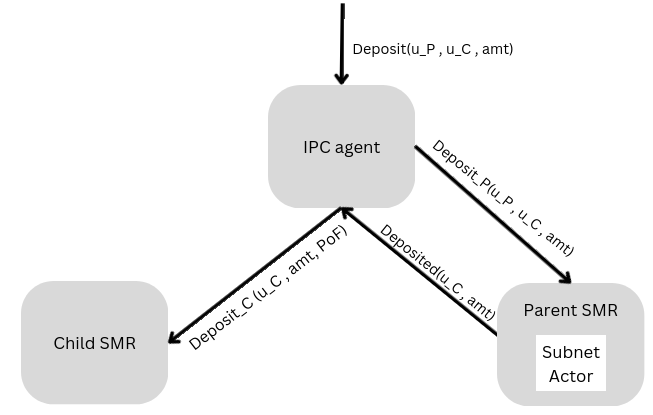
\includegraphics[width=\textwidth]{deposit}
%      \caption{Events produced and consumed during a deposit.}
%      \label{fig:deposit}
% \end{figure}
 

\begin{algorithm}[H]
\footnotesize
\caption{Deposit operation}\label{alg:deposit}
  \DontPrintSemicolon
  \SetKwFunction{FMain}{Global}
  \SetKwProg{Pn}{Function}{:}{\KwRet}
  \SetKwInOut{Input}{input}
  \SetKwProg{Component}{$\blacktriangleright$ \bf}{:}{\KwRet}
  \SetKwFor{UponKW}{upon}{do}{fintq}

   \Component{Owner of \src}{
        submit $\tx=\textit{P.\sa.Deposit}\left( \src, \fil, \dest \right)$ to parent subnet\;
  }
   \Component{P.\sa.Deposit(\src, amt, \dest)}{
    move $\fil$ from \src to P.\sa.\textit{accounts}.\dest  \tcp*[r]{"lock" at parent}
  }
  \Component{IPC agent}{
    \UponKW{tx = P.\sa.Deposit final at parent}{
        create \prf that \tx is final at parent subnet \tcp*[r]{see \cref{sec:finality}}
        submit \textit{P/C.\gw.Deposited(amt, \dest, \pof)}
     }
     \jorge{this notation is also a bit weird, in that "upon tx ... final at parent" is running text and it's not immediately obvious that that's the condition}
  }
  \Component{P/C.\gw.Deposited(amt, \dest, \pof)}{
%    \UponKW{\texttt{Deposited}}{
        verify(\pof)\;
        increase \dest account by \fil
%     }
  }
\end{algorithm}

\subsection{Withdrawals}
\label{sec:withdraw}

A withdrawal is a transfer of funds from an account \src in the child subnet $P/C$ to an account \dest in the parent subnet $P$.
The \emph{Withdraw} is performed analogously to the \emph{Deposit}, but starting at the child subnet $P/C$:
\begin{enumerate}
  \item The owner of \src submits a transaction \emph{tx =} $\textit{P/C.\gw.Withdraw}(\src, \fil, \dest)$.
    \item The child subnet orders and executes the \emph{Withdraw} transaction, burning $\fil$ funds in $\src$ (provided $\src$ has enough funds).
    \item When the child's replicated state that includes the transaction becomes final (for some SMR-system-specific definition of finality that has been defined in the SA), the \ipc agent constructs a corresponding \pof and submits a transaction \textit{\tx' = P.\sa.Withdrawn(\fil, \dest, \pof)} to the parent subnet.
    \item Upon ordering $\tx'$, \emph{P.\sa.Withdrawn(amt, \dest, \pof)} verifies the \pof and transfers \emph{amt} from \sa (concretely, to $\src$ account representation within the \sa) to $\dest$ within the parent subnet.
\end{enumerate}

 % \begin{figure}[h]
 %     \centering
 %     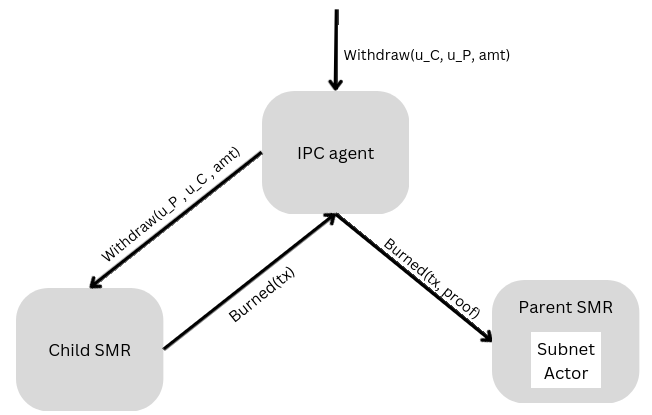
\includegraphics[width=\textwidth]{withdrawal}
 %     \caption{Events produced and consumed during a withdrawal.}
 %     \label{fig:withdrawal}
 % \end{figure}
 We show in Algorithm~\ref{alg:withdraw} the pseudocode to implement the functionality. 

\begin{algorithm}[H]
\footnotesize
\caption{Withdraw operation}\label{alg:withdraw}
  \DontPrintSemicolon
  \SetKwFunction{FMain}{Global}
  \SetKwProg{Pn}{Function}{:}{\KwRet}
  \SetKwInOut{Input}{input}
  \SetKwProg{Component}{$\blacktriangleright$ \bf}{:}{\KwRet}
  \SetKwFor{UponKW}{upon}{do}{fintq}
  % \Input{user~$\user$, amount~$\fil$, transaction \txnf}
   \Component{owner of \src}{
        submit $\tx=\textit{P/C.\gw.Withdraw}(\src, \fil, \dest)$\;
  }
   %
   \Component{\textit{P/C.\gw.Withdraw(\src, \fil, \dest)}}{
    deduct $\fil$ from \src \tcp{"burns" \fil in child}
  }
  \Component{IPC agent}{
    \UponKW{tx = P/C.\gw.Withdraw(\src, \fil, \dest) final at child}{
        create $\pof(tx)$ \tcp*[r]{see \cref{sec:finality} for details}
        submit \textit{P.\sa.Withdrawn(amt, \dest, \pof)}
     }
  }
  \Component{P.\sa.Withdrawn(amt, \dest, \pof)}{
    verify($\pof(tx')$)\;
    move \fil coins from P.\sa to \dest \tcp{"unlocks" \textit{amt} for \dest}
  }
   
\end{algorithm}
\label{enhancedFunc}

\subsection{Checkpointing} 
A checkpoint contains a representation of the state of the child subnet to be included in the parent subnet's replicated state. A checkpoint can be triggered by predefined events (e.g.,  periodically, after a number of state updates, triggered by a specific user or set of users, etc.).
A checkpoint is created as follows:
\begin{enumerate}
    \item When the predefined checkpoint trigger is met (the IPC Agent, monitoring the child subnet's state, is configured with the checkpoint trigger),
    the IPC agent retrieves the corresponding checkpoint data (\emph{chkp}) from the child subnet, along with the proof of its finality (\emph{\pof}).
    \item The IPC agent submits a transaction \emph{tx = P.\sa.Checkpoint(chkp, \pof)}.
    \item The \emph{P.SA.Checkpoint(chkp, \pof)} invocation, after verifying the \emph{\pof}, includes \emph{chkp} in its state.
\end{enumerate}

% \TODO{Pseudocode}
% See commented algorithm

% \begin{figure}[h]
%      \centering
%      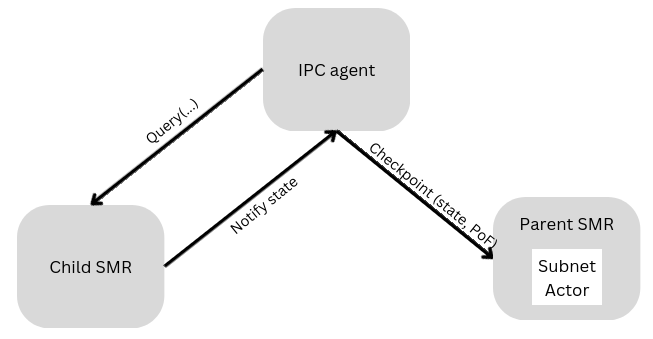
\includegraphics[width=\textwidth]{checkpoint.png}
%      \caption{Events produced and consumed by the checkpointing functionality.}
%      \label{fig:chkp}
%  \end{figure}
Note that we do not show here incentives for participants to submit checkpoints, \add{the same way we do not discuss in Algorithm~\ref{alg:checkpoint} whether the particular participant running the IPC agent has even rights to submit the checkpoint. We show instead in Section~\ref{sec:incentives} different mechanisms that can be used to incentivize participants running IPC agents, while in Section~\ref{sec:ref-impl} we describe how the reference implementation of IPC incentivizes and gives participants the right to submitting checkpoints. Analogously, we discuss in Section~\ref{sec:ref-impl} optimizations and other design decisions made to the checkpoint operation.}



\begin{algorithm}[H]
\footnotesize
\caption{Checkpoint operation}\label{alg:checkpoint}
  \DontPrintSemicolon
  \SetKwFunction{FMain}{Global}
  \SetKwProg{Pn}{Function}{:}{\KwRet}
  \SetKwInOut{Input}{input}
  \SetKwProg{Component}{$\blacktriangleright$ \bf}{:}{\KwRet}
  \SetKwFor{UponKW}{upon}{do}{fintq}

  \Component{IPC agent}{
    \UponKW{Checkpoint condition in child}{
      $chkp = $ obtain state snapshot from child\;
      create $\pof(chkp)$\;
      submit $P.\sa.Checkpoint(chkp, \pof(chkp))$
    }
  }

  \Component{P.\sa.Checkpoint(chkp, \pof(chkp))}{
    verify($\pof(tx')$)\;
    save $chkp$ in the state\;
    % \TODO{Expand on this. check if the checkpoint is the latest one and use a variable to store the latest checkpoint}
  }
   
\end{algorithm}

% OLD PSEUDOCODE
% \begin{algorithm}[H]
% \footnotesize
% \caption{Checkpoint operation\TODO{Update to new terminology}}\label{alg:down}
%   \DontPrintSemicolon
%   \SetKwFunction{FMain}{Global}
%   \SetKwProg{Pn}{Function}{:}{\KwRet}
%   \SetKwInOut{Input}{input}
%   \SetKwProg{Component}{$\blacktriangleright$ \bf}{:}{\KwRet}
%   \SetKwFor{UponKW}{upon}{do}{fintq}
%    \Component{IPC agent}{
%         \If{trigger for checkpoint}{
%             \textit{SA\_state} $\gets$ query parent for \sa's state\;
%             \If{\textit{Self} \textbf{in} SA\_state.validators}{
%                 \textit{state} $\gets$ query child for state\;
%                 \textit{cState} $\gets$ \textit{compressState}(\text{state},\textit{SA\_state.latestCheckpoint})\;
%                 create \prf that \textit{cState} is final at child\;
%             }
%             $\tx=\sa.\texttt{Checkpoint}\left(\textit{cState}, \prf \right)$ \;
%             \If{\textit{Self.}\ssc(tx, SA\_state, ...)}{
%                 submit $tx$ to parent \smr replica\;
%             }
%         }
%   }
%   \Component{parent \smr replica}{
%     \UponKW{$\tx=\sa.\texttt{Checkpoint}\left(\textit{cState}, \prf \right)$}{
%         assert \sa.\verifyGfinal{\textit{cState}}{\prf}\;
%         $\sa.\textit{latestCheckpoint.update}(\textit{cState})$
%      }
%   }
% \end{algorithm}

% The above pseudo code is intentionally abstract, with a number of implementation decisions not specified, such as the main function for creating and verifying a \prf, events that trigger the creation of a new checkpoint, the compression procedure with respect to the previous checkpoint, and the \ssc function to decide whether the participant submits or not a checkpoint. 

% The above pseudo code is highly abstract, with the main function of creating and verifying a \prf not specified. Moreover, other important aspects that are not covered include specific compression mechanisms for the checkpoint data, triggering checkpoints efficiently, and particular incentives for checkpoints creation and submission. \arp{we refer to reference implementation... later in this document we list others...}
% The function \ssc comprises two aspects of the checkpointing functionality from the perspective of participants. First, it controls access to submit checkpoints, as not all subnets will define the same policy to follow when deciding the participants that are allowed to submit checkpoints. Second, it contains the implications of submitting a checkpoint transaction (i.e. the cost involved in being the submitter). For example, if only one transaction is required by any participant but the cost of submitting the checkpoint is incurred on the submitter, then there is a risk of no participant actually submitting the checkpoint if they are strictly rational. An example on the other end might be requiring all participants to submit a transaction for the checkpoint to be finalized at the parent, but this approach affects performance. \arp{We analyze and suggest later in this document multiple mechanisms to ensure through incentives that at least one rational participant will always submit the checkpoint. }

\subsection{Propagating cross-net transactions}
\label{sec:cross-net-tx}

Unlike a "standard" transaction issued and submitted to a subnet by a user,
a cross-net transaction is issued by the replicated logic of another subnet.
Cross-net transactions are a means of interaction between actors located on different subnets.

Since those actors themselves are not processes (but mere parts of a subnet's replicated state),
they cannot directly submit transactions to other subnets.
IPC therefore provides a mechanism to propagate these transactions between subnets using the \postoffice and an IPC agent.
\add{In a nutshell, if an actor's logic in subnet $S_1$ produces a transaction for a different subnet $S_2$,
this transaction is saved at $S_1$'s \gw in the postbox buffer.
The IPC agent, monitoring the \postoffice, then iteratively submits the transaction to the appropriate subnets along the path from $S_1$ to $S_2$.} \del{In a nutshell, if
a actor’s logic produces a transaction for a different subnet, this transaction
is saved the local Gateway Actor in the postbox buffer. The IPC agent,
monitoring the postbox, then submits the transaction to the appropriate
subnet.}

Since, in general, we only rely on IPC Agents to be able to submit transactions to parents or children of a subnet whose state they observe,
the IPC agent only propagates the transaction to the parent or child, depending on which is closer in the IPC hierarchy to the ultimate destination subnet.
After such ``one hop``, the transaction is again placed in the \postoffice of the parent / child, and the process repeats until the transaction reaches its destination subnet.

The implementation of the \gw's \emph{Propagate} function is sketched in \Cref{alg:po}.

\TODO{Outline algorithm in text, like in the rest of functionalities.}

% \guy{Edge case: a leaf subnet does not have a \sa and, therefore, no \postoffice. We can consider removing the \postoffice functionality from the \sa and to deploy it as an independent \actor that will appear only once per subnet. In this case, it needs permissions to call \sa.\verifyGfinal{\tx}{\prf} function.}

\begin{algorithm}[H]
\footnotesize
\caption{Cross-net transaction propagation functionality}\label{alg:po}
  \DontPrintSemicolon
  \SetKwFunction{FPropagate}{propagate}
  \SetKwProg{Pn}{Function}{:}{\KwRet}
  \SetKwInOut{Input}{input}
  \SetKwProg{Component}{$\blacktriangleright$ \bf}{:}{\KwRet}
  \SetKwProg{Empty}{\bf}{:}{\KwRet}
  \SetKwFor{UponKW}{upon}{do}{fintq}
  \Component{\add{S.}\gw.Propagate($\tx, \src, \dest, \pof)$)}{
    verify(\tx.\pof)\;
    \Case{\dest = \src}{
        apply \tx
    }
    \Case{\dest requires going up the tree}{
       $\postoffice \leftarrow \postoffice \cup (\tx, \replace{S/\src}{src.Parent}, \dest)$\;
    }
    \Case{\dest requires going down the tree \add{to child $S_c$}}{
        $\postoffice \leftarrow \postoffice \cup (\tx, \replace{\src/S}{S_c}, \dest)$\;
    }
  }
  \Component{IPC agent}{
    \UponKW{new entry (\tx, \src, \dest) in \replace{parent}{S}.\gw.\postoffice}{
        Create \pof proving that \tx' has indeed been added to the list of cross-net transactions in the subnet\;
        submit \tx', augmented by \emph{\pof}
    }   
    % \jorge{do we need to discuss the matter of implicit execution (or future multisig protocol)? maybe a question for Alfonso}\arp{not here imo (this is not the reference implementation), we discuss it in section \ref\{sec:ref-impl}}
}
\end{algorithm}

\subsection{Slashing}
\label{sec:slash}
Slashing is a penalty imposed on provably malicious validators. When validators of a child subnet misbehave, other participants can report the misbehavior for these malicious validators to get punished (e.g. by losing a previously collateralized amount). Contrary to misbehaviors at a rootnet (a subnet with no parent), where misbehavers sucessfully perform their attack without escrow available, misbehaviors at the child can be resolved at the parent subnet, provided the misbehavers have not left the subnet. For this reason, a slashing is notified first at the parent, and reconciled at the child later on. In particular, a slash on provably malicious validators of a child subnet is performed as follows:
\begin{itemize}
    \item When the IPC agent of a correct participant identifies slashable misbehavior at subnet $P/C$ from a set $\mathcal{M}$ of malicious validators of subnet $P/C$, the IPC agent constructs a \textit{Proof of Misbehavior} (\pom). \item The IPC agent then submits transaction $tx=P.\sa.Slash(\mathcal{M}, \pom)$ at the parent.
    \item The parent subnet, upon ordering and executing $tx$, penalizes the misbehavers and updates the state of $\sa$.
    \item Once the parent's replicated state that includes $tx$ becomes final, the IPC agent constructs a $\pof(tx)$ and submits a transaction $tx'=P/C.\gw.Slashed(\mathcal{M}, \pom, \pof(tx))$ 
    \item The child subnet, upon ordering and executing $tx'$, updates its state to reflect the penalization at the parent. 
    % \arp{This behavior at the child can later be updated to abort if it took place with $tx_C$ and in fact $tx_P'$ will never happen (i.e. attackers were faster and left subnet on time)} 
\end{itemize}
\begin{algorithm}[H] 
\footnotesize
\caption{Slash Functionality}\label{alg:down}
  \DontPrintSemicolon
  \SetKwFunction{FMain}{Global}
  \SetKwProg{Pn}{Function}{:}{\KwRet}
  \SetKwInOut{Input}{input}
  \SetKwProg{Component}{$\blacktriangleright$ \bf}{:}{\KwRet}
  \SetKwFor{UponKW}{upon}{do}{fintq}
  % \Input{-}
  \add{
  \Component{IPC agent}{
     \UponKW{misbehavior from set $\mathcal{M}$ found}{
        Construct \pom($\mathcal{M}$)\;
        submit $tx=P.\sa.Slash(\mathcal{M}, \pom)$ to parent subnet
     }
  }
  \Component{$P.\sa.Slash(\mathcal{M}, \pom)$}{
        verify(\pom)\;
        \tcp*[l]{Update state to reflect punishment to $\mathcal{M}$}
  }
  \Component{IPC agent}{
    \UponKW{$tx=P.\sa.Slash(\mathcal{M}, \pom)$ final at parent}{
             create \prf that \tx is final at parent subnet \tcp*[r]{see \cref{sec:finality}}
             submit $tx'=P/C.\gw.Slashed(\mathcal{M}, \pom, \pof)$
    }
    }
  \Component{$P/C.\gw.Slashed(\mathcal{M}, \pom, \pof)$}{
        verify(\pom, \pof)\;
        \tcp*[l]{Update state to reflect punishment to $\mathcal{M}$}
    }
}
    % \UponKW{\arp{State updated after slashing}}{
    %   \arp{Check child SMR rules are still satisfied, remedy/close otherwise?}
    % }

  % \Component{Parent SMR}{
  %       \UponKW{\slashop submitted by IPC agent}{
  %        Update SA state slashing/excluding participants
  %        Notify SA update to IPC agent
  %       }
  % }
\end{algorithm}

\subsection{Removing a child subnet}
\label{sec:remove}

A child subnet $P/C$ can be removed from its parent $P$ through a transaction invoking $P.\gw.RemoveChild(P/C)$. \add{This transaction effectively deregisters the subnet from the IPC hierarchy. We detail further how to remove a child subnet for the reference implementation in~\cref{sec:ref-impl}.}

% OLD PSEUDOCODE
% \begin{algorithm}[H]
% \footnotesize
% \caption{\postoffice Functionality}\label{alg:po}
%   \DontPrintSemicolon
%   \SetKwFunction{FPropagate}{propagate}
%   \SetKwProg{Pn}{Function}{:}{\KwRet}
%   \SetKwInOut{Input}{input}
%   \SetKwProg{Component}{$\blacktriangleright$ \bf}{:}{\KwRet}
%   \SetKwProg{Empty}{\bf}{:}{\KwRet}
%   \SetKwFor{UponKW}{upon}{do}{fintq}
%   \Input{$\tx = \langle \data, \src, \dest, \prf \rangle$}
%   \Component{\gw.\postoffice}{
%      \UponKW{\postoffice.\propagate(\tx) }{
%        \Case{\dest in current subnet}{
%             \postoffice.\propagate\textit{HERE}(\tx)
%        }
%        \Case{\dest requires going up the tree}{
%             \postoffice.\propagate\textit{UP}(\tx)
%        }
%        \Case{\dest requires going down the tree}{
%             \postoffice.\propagate\textit{DOWN}(\tx)
%        }
%      }
%      \UponKW{\postoffice.\propagate\textit{UP}(\tx) }{
%        \If{\src not from this subnet}{
%             assert \sa.\verifyGfinal{\tx}{\prf}\tcp*[r]{the \sa that corresponds to the child subnet from which \tx comes}
%        }
%        \src.\textit{append(\gw's subnet id)}\tcp*[r]{the i.d. of the current subnet}
%        emit event \gw.\postoffice.UP$\langle \data, \src, \dest \rangle$\;
%        % $\tx \gets \langle \data, \src, \dest \rangle$\;
%        notify agent on \gw.\postoffice.UP$\langle \data, \src, \dest \rangle$
%      }
%      \tcp{\propagate\textit{DOWN}(\tx) is analogous to \propagate\textit{UP}(\tx)}
%      \tcp{\propagate\textit{HERE}(\tx) is trivial}
%   }
%   % \Component{parent \smr process}{
%   %    \UponKW{event \postoffice.UP$\langle \data, \src, \dest \rangle$}{
%   %       $\tx \gets \langle \data, \src, \dest \rangle$\;
%   %       notify agent on \postoffice.UP(\tx)
%   %    }
%   % }
%   \Component{IPC agent}{
%     \UponKW{notification of \gw.\postoffice.UP$\langle \data, \src, \dest \rangle$ from child}{
%         $\tx' \gets$ \gw.\postoffice.UP$\langle \data, \src, \dest \rangle$\;
%         create \prf that \tx' is final at child \smr\;
%         $\tx_\textit{new}\gets\langle \tx', \prf \rangle$\;
%         submit \gw.\postoffice.\propagate($\tx_\textit{new}$) to parent \smr
%     }   
% }
% \end{algorithm}
% \subsection{Atomic Execution}
% TODO
